\documentclass[border=2pt]{standalone}
\usepackage{pgfplots}
\pgfplotsset{compat=1.18}
\usetikzlibrary{arrows.meta,positioning}
\usepackage{newtxtext,newtxmath}
\newcommand{\mbb}{mbb/hand}
\begin{document}
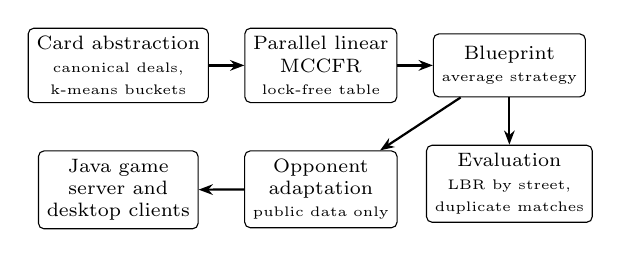
\begin{tikzpicture}[
  box/.style={draw, rounded corners=2pt, align=center, font=\scriptsize, minimum height=0.8cm,
              minimum width=1.9cm, inner sep=3pt},
  arr/.style={-{Stealth[length=1.8mm]}, thick}]
\node[box] (abs) {Card abstraction\\\tiny canonical deals,\\\tiny k-means buckets};
\node[box, right=0.45cm of abs] (mccfr) {Parallel linear\\MCCFR\\\tiny lock-free table};
\node[box, right=0.45cm of mccfr] (bp) {Blueprint\\\tiny average strategy};
\node[box, below=0.6cm of bp] (eval) {Evaluation\\\tiny LBR by street,\\\tiny duplicate matches};
\node[box, below=0.6cm of mccfr] (adapt) {Opponent\\adaptation\\\tiny public data only};
\node[box, below=0.6cm of abs] (server) {Java game\\server and\\desktop clients};
\draw[arr] (abs) -- (mccfr);
\draw[arr] (mccfr) -- (bp);
\draw[arr] (bp) -- (eval);
\draw[arr] (bp) -- (adapt);
\draw[arr] (adapt) -- (server);
\end{tikzpicture}
\end{document}
